% ============================================================================
% FL-EHDS Paper for FLICS 2026 — Condensed 8-page version
% IEEE Conference Format (max 8 pages including references)
% February 2026
% ============================================================================

\documentclass[conference,a4paper]{IEEEtran}

% ===== PACKAGES =====
\usepackage{cite}
\usepackage{amsmath,amssymb,amsfonts}
\usepackage{graphicx}
\usepackage{textcomp}
\usepackage{xcolor}
\usepackage{booktabs}
\usepackage{hyperref}
\usepackage{url}

% TikZ for vector figures
\usepackage{tikz}
\usetikzlibrary{shapes.geometric, arrows.meta, positioning, fit, backgrounds, calc}
\usepackage{pgfplots}
\pgfplotsset{compat=1.18}

% ===== DOCUMENT =====
\begin{document}

\title{FL-EHDS: A Privacy-Preserving Federated Learning Framework for the European Health Data Space}

\author{
    \IEEEauthorblockN{Fabio Liberti}
    \IEEEauthorblockA{
        Department of Computer Science\\
        Universitas Mercatorum, Rome, Italy\\
        fabio.liberti@studenti.unimercatorum.it\\
        ORCID: 0000-0003-3019-5411
    }
}

\maketitle

% ============================================================================
% ABSTRACT
% ============================================================================
\begin{abstract}
The European Health Data Space (EHDS), established by Regulation (EU) 2025/327, mandates cross-border health data analytics while preserving citizen privacy. Federated Learning (FL) is the key enabling technology for secondary use, yet fewer than one in four FL implementations achieve sustained production deployment in healthcare---a gap driven more by legal uncertainty than technical limitations. We present FL-EHDS, a three-layer compliance framework that integrates EHDS governance reference implementations (Health Data Access Bodies, data permits, citizen opt-out registries) with FL orchestration (17 aggregation algorithms including 2024--2025 advances, differential privacy, secure aggregation) and data holder components (adaptive training, FHIR R4 preprocessing). Experimental validation across 1,760+ experiments on tabular clinical and medical imaging datasets---including the European-origin PTB-XL ECG with natural 52-site partitioning---yields two key findings: personalized FL narrows the centralized-federated accuracy gap to 6.6 percentage points (pp) while preserving full data sovereignty, and the architectural choice between personalized and global aggregation dominates over the specific algorithm on clinical tabular models, with five of seven algorithms converging to identical solutions and up to 12.6pp accuracy differences on heterogeneous clinical data. Our evidence synthesis reveals that unresolved regulatory questions---gradient data classification under GDPR, cross-border privacy budget harmonization---constitute the critical adoption blocker rather than technical limitations. The open-source reference implementation provides actionable deployment guidance for the 2029 secondary use deadline.
\end{abstract}

\begin{IEEEkeywords}
Federated Learning, European Health Data Space, Privacy-Preserving Technologies, GDPR, Health Data Governance, Cross-Border Analytics
\end{IEEEkeywords}

% ============================================================================
% 1. INTRODUCTION
% ============================================================================
\section{Introduction}
\label{sec:introduction}

The European Health Data Space (EHDS), established by Regulation (EU) 2025/327, represents the EU's most ambitious initiative for cross-border health data governance~\cite{eu2025ehds}. Entering into force in March 2025, the regulation creates a dual framework: primary use through MyHealth@EU for patient care, and secondary use through HealthData@EU for research, innovation, and policy-making~\cite{ganna2024boost}. Health Data Access Bodies (HDABs) in each Member State authorize secondary use through data permits; Article~53 enumerates permitted purposes; Article~71 introduces citizen opt-out mechanisms~\cite{staunton2024ethical}. The implementation timeline extends to 2031, with delegated acts expected by March 2027 and secondary use provisions applicable from March 2029.

Federated Learning (FL) emerges as the ideal technical solution for EHDS secondary use---the model travels to distributed data rather than centralizing sensitive records~\cite{mcmahan2017communication, kairouz2021advances, rieke2020future}. The COVID-19 pandemic demonstrated FL's potential at scale: Dayan et al.~\cite{dayan2021federated} trained a global model across 20 institutions in 5 countries. However, recent evidence reveals a sobering gap between FL's promise and operational reality. Fr\"ohlich et al.~\cite{frohlich2025reality} report that only 23\% of FL implementations achieve sustained production deployment, with hardware heterogeneity (78\%) and non-IID data distributions (67\%) as dominant barriers. Beyond technical constraints, legal uncertainties regarding gradient data status under GDPR remain unresolved~\cite{quinn2024gdpr}, while van Drumpt et al.~\cite{vandrumpt2025pets} demonstrate that privacy-enhancing technologies cannot substitute for robust governance frameworks.

Prior FL frameworks for healthcare~\cite{rieke2020future, sheller2020federated} focus on technical architectures without addressing regulatory compliance. Legal analyses~\cite{quinn2024gdpr, staunton2024ethical, shabani2024ehds} examine GDPR constraints but abstract from implementation feasibility. Policy documents~\cite{tehdas2024ready} assess Member State readiness but do not integrate FL technical considerations. To our knowledge, no existing work provides an integrated framework addressing all three dimensions: systematic barrier evidence, technical implementation with state-of-the-art algorithms, and EHDS governance operationalization---a gap confirmed by recent systematic reviews of FL frameworks~\cite{kairouz2021advances, teo2024systematic}. Furthermore, no published work experimentally evaluates FL across both tabular EHR and medical imaging modalities within an EHDS-aligned governance architecture with FHIR R4 and OMOP-CDM interoperability.

Our contribution is one of \textit{integration and empirical analysis} rather than novel algorithmic development: we map established FL techniques and privacy mechanisms onto EHDS governance requirements, and through systematic evaluation reveal deployment-critical patterns that no prior work has identified. Specifically:
\begin{enumerate}
    \item \textbf{Evidence Synthesis}: PRISMA-based review of 47 documents with GRADE-CERQual confidence assessment, identifying legal uncertainties---not technical barriers---as the critical adoption blocker.
    \item \textbf{Integration Framework}: A three-layer architecture mapping EHDS governance (HDABs, data permits, Article~71 opt-out) to FL orchestration (17 established algorithms, DP-SGD, secure aggregation) and data holder components (FHIR R4, OMOP-CDM). While individual components employ known techniques, the end-to-end integration---binding regulatory workflows to FL configurations---has no counterpart in existing frameworks. Governance modules operate as simulation backends pending HDAB service availability (2027--2029).
    \item \textbf{Key Empirical Finding}: On clinical tabular models, the architectural choice between personalized and global aggregation \textit{dominates} over specific algorithm selection: five of seven algorithms converge to statistically identical solutions, with only methods maintaining separate local models (Ditto, HPFL) differentiating ($p < 0.005$, 10-seed Wilcoxon). This counterintuitive result simplifies EHDS deployment to a single binary choice.
    \item \textbf{Comprehensive Validation}: 1,760+ experiments across tabular and imaging datasets---including the European-origin PTB-XL ECG with natural 52-site partitioning---with DP ablation ($\varepsilon \in \{1, 5, 10, 50\}$) and Article~71 opt-out simulation. Open-source reference implementation ($\sim$40K lines).\footnote{Available at: \url{https://github.com/FabioLiberti/FL-EHDS-FLICS2026}}
\end{enumerate}

% ============================================================================
% 2. BACKGROUND AND RELATED WORK
% ============================================================================
\section{Background and Related Work}
\label{sec:background}

\subsection{EHDS and Federated Learning}

The EHDS establishes HDABs to authorize secondary use through standardized data permits, with Secure Processing Environments (SPEs) providing controlled analytics settings~\cite{svingel2025hdab}. Forster et al.~\cite{forster2025journeys} document significant variability in data access timelines---from 3 weeks (Finland) to over 12 months (France)---with barriers primarily organizational rather than technical. TEHDAS assessments~\cite{tehdas2024ready} reveal Nordic countries demonstrate 2--3 year advantages in HDAB capacity-building, raising concerns about implementation equity. Teo et al.~\cite{teo2024systematic} and Peng et al.~\cite{peng2024systematic} find that only 5.2\% of FL healthcare studies achieve real-life application.

FL inverts the traditional ML paradigm: local training produces gradients that are aggregated centrally and redistributed~\cite{mcmahan2017communication, li2020federated}. Known challenges include non-IID data distributions causing convergence difficulties~\cite{li2020federated}, communication costs for gradient exchange~\cite{bonawitz2019scale}, and privacy attacks including gradient inversion~\cite{zhu2019deep} and membership inference~\cite{shokri2017membership, carlini2022privacy}. Recent advances from top venues (ICML/ICLR 2022--2025) specifically target healthcare heterogeneity: FedLC~\cite{zhang2022fedlc} calibrates logits for label distribution skew, FedLESAM~\cite{qu2024fedlesam} provides globally-guided sharpness-aware optimization (ICML 2024 Spotlight), and HPFL~\cite{chen2025hpfl} decouples backbone from classifier for per-institution specialization (ICLR 2025).

\subsection{Related Frameworks}

Existing FL frameworks---Flower~\cite{beutel2023flower} (v1.26), NVIDIA FLARE~\cite{nvflare2023} (v2.7), and TensorFlow Federated~\cite{tff2019} (v0.88)---provide robust distributed training but lack EHDS-specific governance. A recent FAIR-based assessment of 17 FL frameworks for biomedical research~\cite{chaverodiez2026fair} confirms that none implements HDAB integration, data permit lifecycle, opt-out enforcement, or audit trails---and identifies limited interoperability as the critical systemic gap. Table~\ref{tab:framework_comparison} provides a detailed comparison.

\begin{table}[htbp]
\centering
\caption{Framework Comparison: FL-EHDS vs Existing FL Frameworks}
\label{tab:framework_comparison}
\resizebox{\columnwidth}{!}{%
\begin{tabular}{lcccc}
\toprule
\textbf{Dimension} & \textbf{FL-EHDS} & \textbf{Flower v1.26} & \textbf{FLARE v2.7} & \textbf{TFF v0.88} \\
\midrule
FL Algorithms & 17 built-in & 12+ strategies & 5 built-in & 3 built-in \\
Byzantine Resilience & 6 methods & 4 methods & --- & --- \\
Differential Privacy & Central+Local & Central+Local & Built-in & Adaptive clip. \\
Secure Aggregation & Pairwise+HE & SecAgg+ & Built-in+HE & Mask-based \\
\midrule
EHDS Governance & \textbf{Full}$^\ddagger$ & None & None & None \\
HDAB Integration & \checkmark$^\ddagger$ & --- & --- & --- \\
Data Permits (Art.~53) & \checkmark$^\ddagger$ & --- & --- & --- \\
Opt-out (Art.~71) & \checkmark$^\ddagger$ & --- & --- & --- \\
Audit Trail (Art.~30) & \checkmark & --- & Audit logs & --- \\
\midrule
Healthcare Stds. & FHIR R4 & MONAI & MONAI & --- \\
Backend & PyTorch & Agnostic & Agnostic & TF only \\
\bottomrule
\end{tabular}%
}

\vspace{1mm}
\footnotesize{$^\ddagger$Reference implementation with simulation backend; production deployment requires binding to actual HDAB services (expected 2027--2029). See Section~\ref{sec:framework} and Supplementary Material, Table~S-IV for readiness assessment.}
\end{table}

\subsection{Evidence Synthesis}

Following PRISMA 2020 guidelines, database searches (PubMed, IEEE Xplore, Scopus, Web of Science, arXiv) identified 847 records; 47 met inclusion criteria (2022--2026, FL/EHDS focus, peer-reviewed or recognized institutional origin). Quality was assessed using MMAT; confidence using GRADE-CERQual (see Supplementary Material, Fig.~S-1 for the complete PRISMA flow diagram). Table~\ref{tab:barriers} summarizes the five dominant barriers with prevalence and mitigation strategies.

\begin{table}[htbp]
\caption{FL Implementation Barriers for EHDS}
\label{tab:barriers}
\centering
\small
\begin{tabular}{p{2.0cm}cp{2.0cm}p{1.8cm}}
\toprule
\textbf{Barrier} & \textbf{Prev.} & \textbf{Evidence} & \textbf{Mitigation} \\
\midrule
Hardware heterog. & 78\% & Fr\"ohlich 2025 & Adaptive engine \\
Non-IID data & 67\% & Multiple & FedProx, Ditto \\
Production gap & 23\% & Fr\"ohlich 2025 & Ref.\ implementation \\
FHIR compliance & 34\% & Hussein 2025 & Preprocessing \\
Communication cost & High & Bonawitz 2019 & Compression \\
\bottomrule
\end{tabular}
\end{table}

Three critical legal questions remain unresolved~\cite{quinn2024gdpr}: (1) whether model gradients constitute ``personal data'' under GDPR, given that gradient inversion attacks demonstrate potential re-identification~\cite{zhu2019deep}; (2) when aggregated models become sufficiently ``anonymous'' to escape GDPR scope; (3) controller/processor allocation in multi-party FL architectures. These legal uncertainties create compliance risks that discourage organizational adoption regardless of technical maturity (GRADE-CERQual: MODERATE).

% ============================================================================
% 3. FL-EHDS FRAMEWORK
% ============================================================================
\section{FL-EHDS Framework}
\label{sec:framework}

Based on the identified barriers, we present FL-EHDS, a three-layer compliance framework for EHDS cross-border health analytics. Figure~\ref{fig:architecture} illustrates the architecture.

\begin{figure*}[t]
\centering
\includegraphics[width=\textwidth]{figures/fig1_composite_final}
\caption{FL-EHDS composite architecture.
(a)~Three-layer compliance framework: Layer~1 (Governance) manages
HDAB integration, data permit authorization, and Article~71 opt-out
registries; Layer~2 (FL Orchestration) operates within the Secure
Processing Environment with gradient aggregation, differential privacy,
and GDPR-compliant audit logging; Layer~3 (Data Holders) implements
local model computation with raw health data never leaving institutional
boundaries. (b)~EHDS interoperability pipeline: heterogeneous sources
across 27 Member States flow through terminology harmonization,
interoperability standards (FHIR~R4, OMOP~CDM, IHE profiles), and
security/compliance layers before reaching the FL training engine.}
\label{fig:architecture}
\end{figure*}

\subsection{Layer 1: Governance}

The reference implementation provides standardized APIs for automated data permit verification before FL training initiation, designed to bind to production HDAB endpoints as they become available (expected 2027--2029). Multi-HDAB synchronization protocols coordinate cross-border studies involving multiple Member States, addressing the coordination complexity identified by Christiansen et al.~\cite{christiansen2025pilot}. National opt-out registries are consulted before each training round, ensuring Article~71 compliance at record-level granularity. Comprehensive audit trails satisfy GDPR Article~30 requirements, documenting data access, processing purposes, and model outputs for regulatory inspection.

Algorithm~1 presents the core FL-EHDS training procedure, highlighting governance checkpoints integrated into each round.

\begin{figure}[htbp]
\centering
\fbox{\parbox{0.92\columnwidth}{
\small
\textbf{Algorithm 1: FL-EHDS FedAvg Training}\\[2pt]
\textbf{Input:} Hospitals $\mathcal{H} = \{h_1, \ldots, h_K\}$, permit $P$, rounds $T$\\
\textbf{Output:} Global model $\theta^{(T)}$\\[3pt]
\textbf{Server executes:}\\
\hspace*{4mm}Initialize $\theta^{(0)}$\\
\hspace*{4mm}\textbf{for} round $t = 1$ to $T$ \textbf{do}\\
\hspace*{8mm}\textit{// Governance check (Layer 1)}\\
\hspace*{8mm}\textbf{if} not ValidatePermit($P$, $t$) \textbf{then abort}\\
\hspace*{8mm}$\mathcal{H}_t \leftarrow$ SelectParticipants($\mathcal{H}$)\\
\hspace*{8mm}\textbf{for each} $h \in \mathcal{H}_t$ \textbf{in parallel do}\\
\hspace*{12mm}$\Delta_h^{(t)}, n_h \leftarrow$ LocalTrain($h$, $\theta^{(t-1)}$)\\
\hspace*{8mm}\textit{// Aggregation with privacy (Layer 2)}\\
\hspace*{8mm}$\theta^{(t)} \leftarrow \theta^{(t-1)} + \frac{1}{\sum n_h} \sum_{h} n_h \cdot \Delta_h^{(t)}$\\
\hspace*{8mm}LogCompliance($t$, $\mathcal{H}_t$)\\[3pt]
\textbf{LocalTrain}($h$, $\theta$):\\
\hspace*{4mm}$\mathcal{D}_h \leftarrow$ FilterOptedOut($\mathcal{D}_h$, Registry) \textit{// Art.~71}\\
\hspace*{4mm}$\theta_h \leftarrow \theta$; train $E$ epochs on $\mathcal{D}_h$\\
\hspace*{4mm}$\Delta_h \leftarrow$ ClipGradient($\theta_h - \theta$, $C$) \textit{// DP bound}\\
\hspace*{4mm}\textbf{return} $\Delta_h$, $|\mathcal{D}_h|$
}}
\end{figure}

\subsection{Layer 2: FL Orchestration}

The framework implements 17 aggregation algorithms spanning six categories (Table~\ref{tab:algo_catalogue})---from foundational methods (FedAvg~\cite{mcmahan2017communication}, FedProx~\cite{li2020federated}) through non-IID robustness (SCAFFOLD~\cite{karimireddy2020scaffold}, FedNova~\cite{wang2020tackling}, FedDyn~\cite{acar2021feddyn}), adaptive optimization~\cite{reddi2021adaptive}, and personalization (Ditto~\cite{li2021ditto}, Per-FedAvg~\cite{fallah2020personalized}) to FedLESAM~\cite{qu2024fedlesam} (ICML 2024) and HPFL~\cite{chen2025hpfl} (ICLR 2025). Composable strategies (FedLC~\cite{zhang2022fedlc}, FedDecorr~\cite{shi2023feddecorr}) can augment any base aggregation.

\begin{table}[htbp]
\centering
\caption{FL-EHDS Algorithm Catalogue (17 Algorithms)}
\label{tab:algo_catalogue}
\small
\begin{tabular}{llll}
\toprule
\textbf{Algorithm} & \textbf{Venue} & \textbf{Category} & \textbf{Key Property} \\
\midrule
FedAvg & AISTATS'17 & Baseline & Weighted avg. \\
FedProx & MLSys'20 & Non-IID & Proximal reg. \\
SCAFFOLD & ICML'20 & Non-IID & Variance red. \\
FedNova & NeurIPS'20 & Non-IID & Normalized avg. \\
FedDyn & ICLR'21 & Non-IID & Dynamic reg. \\
FedAdam & ICLR'21 & Adaptive & Server momentum \\
FedYogi & ICLR'21 & Adaptive & Sparse stability \\
FedAdagrad & ICLR'21 & Adaptive & Grad.\ accum. \\
Ditto & ICML'21 & Personal. & Dual models \\
Per-FedAvg & NeurIPS'20 & Personal. & MAML-based \\
FedLC & ICML'22 & Label skew & Logit calibration \\
FedSAM & ICML'22 & Generalize & Flat minima \\
FedDecorr & ICLR'23 & Represent. & Decorrelation \\
FedSpeed & ICLR'23 & Efficiency & Fewer rounds \\
FedExP & ICLR'23 & Server-side & POCS step size \\
\textbf{FedLESAM} & \textbf{ICML'24} & \textbf{Generalize} & \textbf{Global SAM} \\
\textbf{HPFL} & \textbf{ICLR'25} & \textbf{Personal.} & \textbf{Local classif.} \\
\bottomrule
\end{tabular}

\vspace{1mm}
\footnotesize{\textbf{Bold}: newly added algorithms (2024--2025). All 17 implemented in the open-source reference implementation.}
\end{table}

\textbf{Privacy Protection}: Differential privacy~\cite{dwork2014dp} with configurable $\varepsilon$-budget uses DP-SGD~\cite{abadi2016deep} with R\'enyi DP (RDP)~\cite{mironov2017renyi} for tight composition accounting over multiple training rounds~\cite{wei2020federated}. For Gaussian mechanisms with noise scale $\sigma$, the RDP guarantee at order $\alpha$ is $\rho(\alpha) = \alpha/(2\sigma^2)$. For 100+ round training typical of EHDS cross-border studies, RDP provides 5--6$\times$ tighter privacy bounds than naive composition~\cite{mironov2017renyi, wei2020federated}, enabling longer training with equivalent privacy guarantees. Gradient clipping bounds individual contributions; secure aggregation (pairwise masking protocol with ECDH key exchange) mitigates gradient inversion attacks~\cite{zhu2019deep}. Six Byzantine resilience methods (Krum, Multi-Krum, Trimmed Mean, Median, Bulyan, FLTrust) defend against up to $f < n/3$ malicious clients.

\textbf{Purpose Limitation}: Technical enforcement of Article~53 permitted purposes through model output filtering and use-case validation, preventing scope creep beyond authorized analytics.

\subsection{Layer 3: Data Holders}

Resource-aware training engines address hardware heterogeneity (78\% barrier prevalence). The engine dynamically adjusts batch sizes, model complexity, and synchronization frequency based on local computational capabilities, enabling participation of institutions with diverse hardware profiles---from GPU-equipped university hospitals to CPU-only rural clinics.

\textbf{FHIR Preprocessing}: Data normalization pipelines ensure interoperability across heterogeneous EHR systems. Only 34\% of European healthcare providers achieve full FHIR compliance~\cite{hussein2025interop}; the preprocessing module bridges format gaps through automated transformation pipelines supporting FHIR R4 resources (Patient, Observation, Condition, MedicationRequest, DiagnosticReport) with standard coding systems (SNOMED-CT, LOINC, ICD-10).

\textbf{Secure Communication}: End-to-end encrypted gradient transmission with certificate-based authentication ensures no raw data leaves institutional boundaries. The communication layer supports gRPC for model updates and WebSocket for real-time monitoring events.

\subsection{Threat Model}

We consider three adversary classes: \textit{(i)~honest-but-curious server}, mitigated by central DP ($\varepsilon \in \{1{,}5{,}10{,}50\}$, $\delta{=}10^{-5}$) with R\'enyi composition and secure aggregation; \textit{(ii)~malicious clients} ($f < n/3$), mitigated by Byzantine-resilient aggregation (Krum, Trimmed Mean, Bulyan); \textit{(iii)~external attackers}, mitigated by Article~71 output filtering and HDAB permit-based access control. Raw patient data never leaves institutional boundaries. Server-client collusion and side-channel attacks remain out of scope (see Supplementary Material for full security analysis).

\subsection{EHDS Compliance Mapping}

Table~\ref{tab:compliance} maps framework components to EHDS regulatory requirements.

\begin{table}[htbp]
\caption{EHDS Compliance Mapping}
\label{tab:compliance}
\centering
\small
\begin{tabular}{lp{2.3cm}p{2.8cm}}
\toprule
\textbf{Article} & \textbf{Requirement} & \textbf{FL-EHDS Component} \\
\midrule
Art. 33 & Secondary use auth. & HDAB API + Permit valid. \\
Art. 46 & Cross-border proc. & Multi-HDAB coordinator \\
Art. 50 & Secure Proc.\ Env. & Aggregation within SPE \\
Art. 53 & Permitted purposes & Purpose limitation module \\
Art. 71 & Opt-out mechanism & Registry filtering \\
\bottomrule
\end{tabular}
\end{table}

\subsection{Reference Implementation}

A modular Python implementation is available as open-source software, designed following FAIR principles~\cite{chaverodiez2026fair} (findable via GitHub with DOI, accessible under MIT license, interoperable via PyTorch and FHIR R4 interfaces, reusable with comprehensive documentation). The codebase ($\sim$40K lines, 159 modules) provides: (1) orchestration modules implementing all 17 algorithms with RDP accounting and secure aggregation; (2) six Byzantine resilience methods; (3) data holder utilities for adaptive training and FHIR R4 preprocessing; (4) a Streamlit-based dashboard for interactive FL training, EHDS governance workflow, and real-time monitoring; (5) a professional terminal UI with 11 specialized screens; (6) reproducible benchmark suite generating all experimental results.

\textbf{Note on governance maturity}: HDAB integration, data permits, and Article~71 opt-out are implemented as simulation backends (OAuth2/mTLS, permit CRUD, cross-border coordination). These modules require only configuration changes (endpoint URLs, certificates) for production binding to actual HDAB services (expected 2027--2029). Readiness assessment in Supplementary Material, Table~S-IV.

% ============================================================================
% 4. EXPERIMENTAL EVALUATION
% ============================================================================
\section{Experimental Evaluation}
\label{sec:experiments}

We evaluate FL-EHDS on real clinical datasets simulating cross-border healthcare analytics. All results are fully reproducible via the benchmark suite in the repository.

\subsection{Setup}

\textbf{Datasets}: We evaluate on 8 datasets spanning tabular EHR and medical imaging (Table~\ref{tab:dataset_coverage}). Tabular datasets cover three scale regimes: \textit{small-data FL} (Heart Disease UCI, 920 patients from 4 international hospitals with natural non-IID partitioning; Breast Cancer Wisconsin, 569 FNA pathology samples), \textit{medium-scale} (PTB-XL ECG~\cite{wagner2020ptbxl}, 21,799 European-origin records from 52 German recording sites with natural hospital partitioning and 5-class SCP-ECG diagnosis), and \textit{large-scale} (Diabetes 130-US~\cite{strack2014diabetes}, 101,766 encounters; Cardiovascular Disease, 70,000 patients). Imaging datasets include Chest X-ray (5,856, binary), Brain Tumor MRI (7,023, 4-class), and Skin Cancer (3,297, binary). The full 19-dataset framework landscape is detailed in Supplementary Material, Table~S-I. \textbf{Model}: HealthcareMLP (2-layer, 64/32 hidden, ReLU, dropout 0.3, $\sim$2.9K--10K parameters depending on input dimensionality) for tabular; ResNet-18 ($\sim$11.2M parameters) for imaging. \textbf{Configuration}: Per-dataset optimized hyperparameters (see Supplementary Material, Table~S-XV): PTB-XL (lr=0.005, bs=64, 30 rounds), Cardiovascular (lr=0.01, bs=64, 25 rounds), Breast Cancer (lr=0.001, bs=16, 40 rounds, 1 local epoch to prevent overfitting on 569 samples). All other datasets use 3 local epochs. Adam optimizer throughout; early stopping with patience=6. Tabular baselines: mean $\pm$ std over 5 seeds (10 seeds for significance testing, 3 for scalability); imaging: 3 seeds (Chest X-ray, Skin Cancer) or 1 seed (Brain Tumor).

\begin{table}[htbp]
\centering
\caption{Evaluated Dataset Coverage}
\label{tab:dataset_coverage}
\resizebox{\columnwidth}{!}{%
\begin{tabular}{lcccl}
\toprule
\textbf{Dataset} & \textbf{Samples} & \textbf{Feat.} & \textbf{Cls.} & \textbf{FL Partition} \\
\midrule
\multicolumn{5}{l}{\textit{Tabular Clinical (MLP, $\sim$2.9K--10K params)}} \\
Heart Disease UCI & 920 & 13 & 2 & Natural (4 hosp.) \\
Breast Cancer Wisc. & 569 & 30 & 2 & Dirichlet \\
PTB-XL ECG$^\dagger$ & 21,799 & 9 & 5 & Natural (52 sites) \\
Diabetes 130-US & 101,766 & 22 & 2 & Dirichlet \\
Cardiovascular & 70,000 & 11 & 2 & Dirichlet \\
\midrule
\multicolumn{5}{l}{\textit{Medical Imaging (ResNet-18, $\sim$11.2M params)}} \\
Chest X-ray & 5,856 & --- & 2 & Dirichlet \\
Brain Tumor MRI & 7,023 & --- & 4 & Dirichlet \\
Skin Cancer & 3,297 & --- & 2 & Dirichlet \\
\bottomrule
\end{tabular}%
}

\vspace{1mm}
\footnotesize{$^\dagger$European-origin (PTB, Berlin), SCP-ECG standard (EN 1064), 5-class cardiac diagnosis. The 52 recording sites are grouped into $K$ geographic clusters for FL experiments (default $K{=}5$); client scaling evaluates $K \in \{3, 5, 10, 20\}$ in Supplementary Material.}
\end{table}

\subsection{Algorithm Comparison}

Table~\ref{tab:tabular_main} presents the primary evaluation: 7 algorithms (including FedLESAM and HPFL) on PTB-XL ECG, Cardiovascular, and Breast Cancer. On two additional datasets---Heart Disease (4 natural hospitals, Ditto 75.1\% vs.\ FedAvg 62.5\%, 12.6pp gap) and Diabetes (5 clients, Ditto 71.7\%)---the personalization advantage is confirmed (Supplementary Material, Table~S-VI). Together, 1,760+ experiments span heterogeneity sweeps, client scaling, differential privacy ablation, Article~71 opt-out simulation, and 10-seed statistical validation.

\begin{table*}[htbp]
\centering
\caption{Extended FL Algorithm Comparison on Tabular Healthcare Datasets (7 Algorithms $\times$ 3 Datasets). Best accuracy per dataset in \textbf{bold}. Mean $\pm$ std over 5 seeds. PX = PTB-XL ECG (5 clients, 5-class, site-based), CV = Cardiovascular (5 clients, binary, $\alpha$=0.5), BC = Breast Cancer (3 clients, binary, $\alpha$=0.5).}
\label{tab:tabular_main}
\resizebox{\textwidth}{!}{%
\begin{tabular}{lccccccccc}
\toprule
\textbf{Algorithm} & \multicolumn{3}{c}{\textbf{PTB-XL ECG (21,799 records, 52 sites)}} & \multicolumn{3}{c}{\textbf{Cardiovascular (70K patients)}} & \multicolumn{3}{c}{\textbf{Breast Cancer (569 samples)}} \\
\cmidrule(lr){2-4}\cmidrule(lr){5-7}\cmidrule(lr){8-10}
 & Acc (\%) & F1 (\%) & Jain & Acc (\%) & F1 (\%) & Jain & Acc (\%) & F1 (\%) & Jain \\
\midrule
FedAvg & 91.9$\pm$0.5 & 100.0 & 0.999 & 71.1$\pm$1.8 & 68.8 & 0.981 & 52.3$\pm$17.9 & 32.0 & 0.608 \\
FedProx & 91.6$\pm$0.7 & 100.0 & 0.999 & 71.5$\pm$1.2 & 69.6 & 0.986 & 52.3$\pm$17.9 & 32.0 & 0.608 \\
\textbf{Ditto} & 91.8$\pm$0.3 & 99.3 & 0.999 & \textbf{82.5$\pm$4.7} & 82.3 & 0.980 & \textbf{79.1$\pm$12.5} & 64.5 & 0.606 \\
FedLC & 91.9$\pm$0.5 & 100.0 & 0.999 & 71.1$\pm$1.6 & 68.8 & 0.982 & 52.1$\pm$18.1 & 32.6 & 0.606 \\
FedExP & 92.0$\pm$0.2 & 100.0 & 0.999 & 71.1$\pm$1.8 & 68.8 & 0.981 & 52.3$\pm$17.9 & 32.0 & 0.608 \\
FedLESAM & 91.9$\pm$0.5 & 100.0 & 0.999 & 71.1$\pm$1.8 & 68.8 & 0.981 & 52.3$\pm$17.9 & 32.0 & 0.608 \\
\textbf{HPFL} & \textbf{92.5$\pm$0.3} & 100.0 & 0.999 & 82.3$\pm$4.5 & 82.0 & 0.984 & 74.1$\pm$20.9 & 62.1 & 0.867 \\
\bottomrule
\end{tabular}%
}
\par{\footnotesize F1: positive-class for binary tasks (CV, BC); NORM-class one-vs-rest for PTB-XL (5-class)---the near-100\% values indicate all algorithms classify the majority class correctly, making accuracy and Jain the primary discriminative metrics. BC std reflects single-class collapse (see item~6 below and Supplementary Table~S-XX).}
\end{table*}

\subsection{Convergence and Baselines}

Figure~\ref{fig:convergence} shows training convergence on Heart Disease. Ditto converges faster and higher due to personalized local models. Comprehensive convergence curves for all 7 algorithms across PTB-XL, Cardiovascular, and Breast Cancer are provided in Supplementary Material, Fig.~S-19.

\begin{figure}[htbp]
\centering
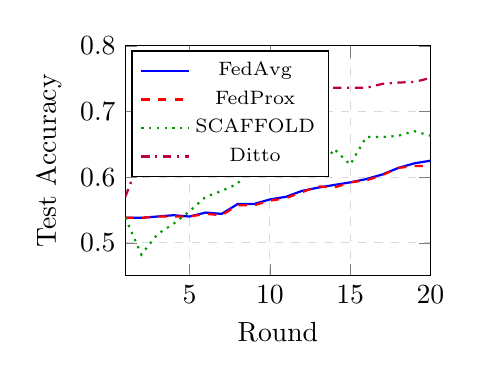
\begin{tikzpicture}
\begin{axis}[
    width=0.45\textwidth,
    height=4.5cm,
    xlabel={Round},
    ylabel={Test Accuracy},
    legend style={at={(0.02,0.98)}, anchor=north west, font=\scriptsize},
    grid=major,
    grid style={dashed, gray!30},
    xmin=1, xmax=20,
    ymin=0.45, ymax=0.80,
]
\addplot[blue, thick] coordinates {(1,0.538) (2,0.538) (3,0.540) (4,0.542) (5,0.540) (6,0.546) (7,0.544) (8,0.559) (9,0.559) (10,0.566) (11,0.570) (12,0.579) (13,0.584) (14,0.588) (15,0.592) (16,0.597) (17,0.604) (18,0.614) (19,0.621) (20,0.625)};
\addplot[red, thick, dashed] coordinates {(1,0.538) (2,0.538) (3,0.540) (4,0.540) (5,0.540) (6,0.544) (7,0.542) (8,0.557) (9,0.557) (10,0.564) (11,0.568) (12,0.577) (13,0.586) (14,0.584) (15,0.592) (16,0.595) (17,0.603) (18,0.614) (19,0.617) (20,0.617)};
\addplot[green!60!black, thick, dotted] coordinates {(1,0.538) (2,0.482) (3,0.513) (4,0.529) (5,0.548) (6,0.570) (7,0.579) (8,0.590) (9,0.625) (10,0.636) (11,0.628) (12,0.626) (13,0.604) (14,0.643) (15,0.619) (16,0.661) (17,0.661) (18,0.663) (19,0.670) (20,0.663)};
\addplot[purple, thick, dashdotted] coordinates {(1,0.570) (2,0.634) (3,0.667) (4,0.689) (5,0.696) (6,0.692) (7,0.705) (8,0.705) (9,0.712) (10,0.722) (11,0.727) (12,0.731) (13,0.736) (14,0.736) (15,0.736) (16,0.736) (17,0.742) (18,0.744) (19,0.745) (20,0.751)};
\legend{FedAvg, FedProx, SCAFFOLD, Ditto}
\end{axis}
\end{tikzpicture}
\caption{Training convergence on Heart Disease UCI (4 hospitals, natural non-IID). Ditto converges faster due to personalized local models. HPFL and FedLESAM convergence curves for all datasets in Supplementary Material, Fig.~S-19.}
\label{fig:convergence}
\end{figure}

\textbf{Key findings}: Ditto converges to 75.1\% by round 20, compared to 62.5\% for FedAvg---a 12.6pp advantage. SCAFFOLD exhibits high variance (oscillating between 48\% and 66\%) due to control variate instability with only 4 heterogeneous clients. FedProx closely tracks FedAvg, suggesting that proximal regularization alone is insufficient for the degree of heterogeneity present.

Table~\ref{tab:fl_vs_central} compares three learning paradigms on Heart Disease, representing the EHDS deployment spectrum: centralized (upper bound, no privacy), federated (data stays local), and local-only (no collaboration).

\begin{table}[htbp]
\centering
\caption{Learning Paradigm Comparison (Heart Disease UCI)}
\label{tab:fl_vs_central}
\small
\begin{tabular}{lcccc}
\toprule
\textbf{Approach} & \textbf{Acc.} & \textbf{F1} & \textbf{AUC} & \textbf{Gap} \\
\midrule
Centralized & $81.7 \pm 2.9$\% & $.815$ & $.882$ & --- \\
FL-Ditto & $75.1 \pm 2.0$\% & $.761$ & $.826$ & 6.6pp \\
FL-FedAvg & $62.5 \pm 8.0$\% & $.736$ & $.834$ & 19.2pp \\
Local-Only$^*$ & $81.7 \pm 1.2$\% & $.797$ & --- & 0.0pp \\
\bottomrule
\end{tabular}

\vspace{1mm}
\footnotesize{4 hospitals, natural non-IID partitioning. Centralized/Local: 60 epochs, Adam (lr=0.01). FL: 20 rounds $\times$ 3 local epochs. Mean $\pm$ std over 5 seeds. $^*$Local-only evaluated on own test split (not cross-hospital).}
\end{table}

FL-Ditto narrows the centralized--federated gap to only \textbf{6.6pp} (75.1\% vs.\ 81.7\%) while preserving full data sovereignty. FedAvg suffers a 19.2pp gap, underscoring the importance of personalization. Local-Only accuracy (81.7\%) appears competitive but is misleadingly evaluated on each hospital's own test split; local models do not generalize across hospitals---precisely the scenario EHDS Article~33 addresses through federated knowledge sharing.

\subsection{Non-IID Impact Analysis}

Figure~\ref{fig:noniid_impact} illustrates the impact of data heterogeneity on algorithm performance. As non-IID severity increases ($\alpha \to 0$), algorithm selection becomes increasingly critical---variance-reduction methods maintain stability while baseline FedAvg degrades significantly.

\begin{figure}[htbp]
\centering
\includegraphics[width=0.95\columnwidth]{figures/fig_accuracy_vs_noniid.pdf}
\caption{Final accuracy vs.\ data heterogeneity level (Dirichlet $\alpha$). Algorithm choice becomes critical as non-IID severity grows.}
\label{fig:noniid_impact}
\end{figure}

\subsection{Key Findings}

\begin{enumerate}
    \item \textbf{Algorithm choice matters}: up to 18.7pp accuracy gap between best (Ditto, 75.1\%) and worst (FedNova, 56.4\%) on Heart Disease; FedNova and SCAFFOLD exhibit known failure modes on class-imbalanced tabular data (see Discussion). Excluding these, personalized methods still dominate: 12.6pp on Heart Disease (Ditto vs.\ FedAvg), 11.4pp on Cardiovascular (Ditto 82.5\% vs.\ FedAvg 71.1\%).

    \item \textbf{Personalization dominates across scales}: HPFL (ICLR 2025) and Ditto consistently outperform baseline algorithms on all datasets. On Breast Cancer---a challenging small-data regime (569 samples, 3 clients)---Ditto achieves 79.1\% vs.\ FedAvg 52.3\% (26.8pp gap). HPFL uniquely improves fairness (Jain 0.867 vs.\ 0.608), reducing the inter-client performance gap from 71.5\% to 47.6\%. Extended 10-seed validation confirms statistical significance: HPFL outperforms FedAvg on all three datasets ($p{=}0.004$, $0.002$, $0.031$; Wilcoxon signed-rank), and Ditto on Cardiovascular and Breast Cancer ($p{=}0.002$, $0.016$). Pooled across 30 observations, both achieve $p < 0.001$.

    \item \textbf{PTB-XL validates European FL}: The European-origin PTB-XL dataset with natural 52-site partitioning achieves 92.5\% accuracy (HPFL) for 5-class ECG diagnosis with near-perfect fairness (Jain 0.999)---demonstrating FL viability for real European multi-center clinical data.

    \item \textbf{Heterogeneity amplifies algorithm differences}: Under extreme non-IID ($\alpha{=}0.1$), Ditto and HPFL \textit{improve} on Cardiovascular (92.4\% vs.\ 82.5\% at $\alpha{=}0.5$) while FedAvg degrades to 61.2\%. This counter-intuitive result confirms that personalized methods exploit heterogeneity rather than suffering from it (see Supplementary Material, Table~S-VII).

    \item \textbf{Personalization architecture is the critical design choice}: On compact tabular models ($\leq$10K parameters), five of seven algorithms (FedLESAM, FedExP, FedLC, FedProx, FedAvg) converge to statistically identical solutions. Only methods maintaining separate local models (Ditto, HPFL) differentiate. This simplifies EHDS deployment decisions: for lightweight clinical models, the choice is between personalized vs.\ global architecture, not among aggregation strategies.

    \item \textbf{Privacy imposes negligible utility cost at $\varepsilon{=}10$}: Ablation across $\varepsilon \in \{1, 5, 10, 50\}$ (180 experiments) reveals that personalized methods are DP-robust: at $\varepsilon{=}10$, Ditto and HPFL lose $<$1pp on PTB-XL (Table~\ref{tab:dp_mini}), while FedAvg collapses ($-$39.6pp at $\varepsilon{=}1$). On the small Breast Cancer dataset (569 samples, 3 clients), an intriguing effect emerges: FedAvg with $\varepsilon{=}5$ achieves 78.7\% vs.\ 52.3\% without DP. This apparent ``noise-as-regularization'' effect should be interpreted cautiously---the no-DP baseline is in single-class collapse, so Gaussian noise disrupts degenerate convergence rather than providing conventional regularization.

    \item \textbf{Article~71 opt-out is compatible with FL quality}: Simulating citizen opt-out at 5--30\% rates (225 experiments) confirms $<$1pp accuracy loss on adequately-sized datasets. However, HPFL shows vulnerability on small datasets ($-$10.4pp at $\geq$10\% opt-out); data permits for personalized methods should specify minimum per-client sample thresholds (full results in Supplementary Material).

    \item \textbf{Modality-dependent personalization}: Tabular FL requires only 0.04~MB/round; imaging (ResNet-18, 11.2M params) requires 44.7~MB/round. Top-$k$ sparsification at 5\% achieves 95\% bandwidth savings but incurs $-$13.4pp accuracy cost on the $\sim$2.9K-parameter tabular MLP (PTB-XL)---the model is too small to tolerate aggressive pruning, as most parameters carry non-redundant information. For imaging models with $>$11M parameters, Top-$k$ is practical (Supplementary Material, Table~S-XXII). Chest X-ray~\cite{chestxray2018} with ResNet-18~\cite{he2016deep}, GroupNorm, and FedBN~\cite{li2021fedbn} achieves 87.3\% (FedAvg). \textbf{Our limited imaging evaluation suggests personalization offers no advantage}: HPFL achieves only 69.1\% on Chest X-ray ($-$18.2pp, 3 seeds); on Skin Cancer (3 seeds), FedAvg and HPFL are statistically indistinguishable (63.0$\pm$9.2\% vs.\ 62.9$\pm$7.5\%), though HPFL maintains superior fairness (Jain 0.971 vs.\ 0.836); on Brain Tumor (1 seed) both achieve $\sim$46\% (Supplementary Material, Table~S-XXV). On tabular Breast Cancer, confusion matrix analysis (10 seeds) confirms HPFL avoids single-class collapse (78.7\% Malignant recall vs.\ 21.5\% for FedAvg; Table~S-XX). EHDS data permits should condition algorithm selection on analytics modality.
\end{enumerate}

\begin{table}[htbp]
\centering
\caption{Privacy-utility on PTB-XL ECG: accuracy (\%) under central DP. Gaussian mechanism, $C{=}1.0$, $\delta{=}10^{-5}$. Mean over 5 seeds.}
\label{tab:dp_mini}
\small
\begin{tabular}{lccc}
\toprule
\textbf{Algorithm} & $\boldsymbol{\varepsilon{=}1}$ & $\boldsymbol{\varepsilon{=}10}$ & \textbf{No DP} \\
\midrule
FedAvg & 52.3 & \textbf{92.4} & 91.9 \\
Ditto & 89.2 & 91.6 & 91.8 \\
HPFL & 87.1 & 92.4 & 92.5 \\
\bottomrule
\end{tabular}
\end{table}

% ============================================================================
% 5. DISCUSSION
% ============================================================================
\section{Discussion}
\label{sec:discussion}

\subsection{Legal Uncertainties as Critical Blocker}

Our synthesis reveals that \textbf{legal uncertainties---not technical barriers---constitute the critical blocker} for FL adoption in EHDS contexts. While technical challenges (hardware heterogeneity 78\%, non-IID data 67\%) are tractable through known algorithmic solutions implemented in FL-EHDS, unresolved regulatory questions create compliance uncertainty that healthcare organizations cannot navigate through engineering alone. Without clarification of gradient data status, organizations face potential GDPR violations regardless of technical privacy measures. This aligns with van Drumpt et al.'s~\cite{vandrumpt2025pets} conclusion that governance frameworks are prerequisites, not alternatives, to technical solutions---synthetic data approaches face similar governance gaps~\cite{jordon2022synthetic}.

A concrete example illustrates this impasse: a German hospital ($\varepsilon_{\max}{=}1.0$, strict BDSG interpretation) federating with an Italian hospital ($\varepsilon_{\max}{=}5.0$, Garante guidance) faces three problematic options: (a)~applying the strictest bound wastes utility (FedAvg collapses from 91.9\% to 52.3\% at $\varepsilon{=}1$); (b)~applying the most permissive risks GDPR sanctions; (c)~per-client $\varepsilon$ introduces asymmetric noise, biasing the global model. FL-EHDS supports per-client privacy budgets, but the policy question---which bound governs---requires regulatory clarification. Article~50(4) mandates that SPEs provide ``a high level of security'' without specifying whether privacy budgets should be harmonized across Member States. The March 2027 delegated acts should address: (1)~gradient data status under GDPR; (2)~controller/processor determination; (3)~anonymization thresholds for aggregated models; (4)~cross-border privacy budget harmonization within SPEs.

\subsection{Experimental Insights for EHDS Deployment}

Our results carry four implications for EHDS deployment. \textit{First}, algorithm gaps up to 12.6pp (excluding known failure modes) demonstrate that EHDS data permits must specify algorithm selection---FL cannot be treated as a black box. \textit{Second}, SCAFFOLD and FedNova fail catastrophically on class-imbalanced tabular data: SCAFFOLD's control variates overcorrect under severe label skew with few heterogeneous clients, while FedNova's normalized averaging amplifies noise from divergent local objectives~\cite{karimireddy2020scaffold, wang2020tackling}; EHDS delegated acts should mandate algorithm validation protocols. \textit{Third}, personalized FL achieves $p < 0.001$ (pooled Wilcoxon, 10-seed) against FedAvg, with HPFL being the only algorithm significantly outperforming FedAvg on all three tabular datasets individually. This aligns naturally with EHDS data sovereignty: each institution retains a locally fine-tuned model while contributing to collective knowledge. \textit{Fourth}, on compact tabular models only methods maintaining \textit{separate local models} (Ditto, HPFL) differentiate, simplifying deployment to a single architectural choice (personalized vs.\ global).

\subsection{Multi-Modal EHDS Coverage}

FL-EHDS is, to our knowledge, the first FL framework providing experimental evaluation across both tabular EHR and medical imaging within an EHDS-aligned governance architecture integrating FHIR R4 and OMOP-CDM interoperability. This dual coverage reveals fundamental design trade-offs: tabular models ($\leq$10K params) incur minimal communication overhead (0.04~MB/round), while imaging models ($\sim$11.2M params) impose 1,000$\times$ higher costs. Crucially, our preliminary imaging evaluation suggests a \textbf{modality-dependent effect}: Ditto/HPFL dominate on tabular data (+12--22pp) but appear counterproductive on Chest X-ray ($-$18.2pp, 3 seeds) and statistically indistinguishable on Skin Cancer and Brain Tumor---though limited seed counts preclude definitive conclusions, requiring EHDS algorithm recommendations to be conditioned on analytics modality. The framework validates FL across three data-scale regimes (569--101K samples), five clinical domains, and both binary and multiclass tasks.

\subsection{Stakeholder Recommendations}

\textbf{EU Policymakers}: The March 2027 delegated acts should address gradient privacy status, controller/processor determination, and cross-border privacy budget harmonization. \textbf{National Authorities}: Early HDAB capacity investment is essential; the 2--3 year Nordic advantage~\cite{tehdas2024ready} demonstrates that governance capacity may prove more constraining than technical infrastructure. \textbf{Healthcare Organizations}: Preparation cannot wait for 2029---accelerating FHIR compliance beyond the 34\% baseline~\cite{hussein2025interop} and assessing FL infrastructure readiness are immediate priorities.

\textit{Practical deployment scenario}: A cardiology consortium of 50 hospitals across three Member States would: (1)~apply for data permits through respective HDABs specifying ``HPFL'' as the FL algorithm with $\varepsilon{=}10$---our experiments confirm $<$1pp accuracy cost even at $K{=}50$; (2)~deploy FL-EHDS data holder components at each hospital with FHIR R4 preprocessing; (3)~execute 25 rounds of federated training within the SPE ($\sim$1~MB total communication for tabular models); (4)~each hospital retains its personalized local model for clinical decision support. The entire process requires no raw data transfer across borders, achieves 82.3\% accuracy on cardiovascular risk prediction under full $\varepsilon{=}10$ privacy, and preserves cross-site fairness (Jain~0.951).

\subsection{Limitations}

\textbf{Dataset}: Our evaluation uses retrospective public datasets; real-world integration with production EHR systems remains essential future work. While PTB-XL provides authentic European multi-site heterogeneity (52 sites), true cross-border validation requires datasets spanning multiple Member States with distinct national healthcare systems---a resource that does not yet exist publicly and that the EHDS itself aims to enable.

\textbf{Evaluation}: The tabular MLP ($\sim$2.9K--10K params) produces a nearly convex loss landscape where server-side strategies converge to FedAvg-equivalent solutions. Confusion matrix analysis (10 seeds) confirms clinically severe single-class collapse on Breast Cancer for all non-HPFL methods (Supplementary Material, Table~S-XX). A deeper model ($\sim$110K params, 4 hidden layers) does \textit{not} break this pattern, nor does increasing local epochs from $E$=1 to $E$=20; however, architectures with BatchNorm or attention layers could introduce non-convexities that differentiate server-side strategies---this remains to be tested. Scalability experiments ($K{=}100$) show the personalization gap \textit{widening} (11.7pp$\to$15.9pp; Tables~S-XVIII--S-XIX). DP at $\varepsilon{=}10$ imposes $<$0.4pp cost across all algorithms, extending to deployment scale $K{=}50$ (Table~S-XXIII). On imaging ($n{=}3$ seeds for Chest X-ray and Skin Cancer, $n{=}1$ for Brain Tumor), HPFL appears counterproductive on Chest X-ray but indistinguishable from FedAvg on Skin Cancer and Brain Tumor; these limited sample sizes preclude statistical significance, and extended multi-seed analysis with additional architectures is deferred.

\textbf{Framework}: The governance layer operates as a simulation backend; binding to actual HDAB REST/gRPC endpoints requires only configuration changes (endpoint URLs, mTLS certificates), not architectural modifications.

% ============================================================================
% 6. CONCLUSIONS
% ============================================================================
\section{Conclusions}
\label{sec:conclusions}

This paper presents FL-EHDS, a three-layer integration framework mapping established FL techniques and privacy mechanisms onto EHDS governance requirements---the first such end-to-end system, though governance modules currently operate as simulation backends pending HDAB service availability (2027--2029). Our most significant empirical finding is that, on clinical tabular models, the architectural choice between personalized and global aggregation \textit{dominates} over specific algorithm selection: five of seven algorithms converge to identical solutions, reducing EHDS deployment decisions to a single binary choice. Validation across 1,760+ experiments further demonstrates: (1)~personalized FL (Ditto, HPFL) narrows the centralized--federated gap to 6.6pp while preserving full data sovereignty ($p < 0.001$, pooled Wilcoxon); (2)~DP at $\varepsilon{=}10$ imposes $<$2pp cost from $K{=}5$ to $K{=}50$, imposing negligible privacy cost; (3)~Article~71 opt-out up to 30\% has negligible impact on adequately-sized datasets.

Our evidence synthesis reveals that legal uncertainties---not technical barriers---constitute the critical adoption blocker. The 23\% production deployment rate~\cite{frohlich2025reality} will not improve through engineering advances alone: concrete governance deadlocks require explicit regulatory guidance in the March 2027 delegated acts. Without this, the 2029 secondary use deadline arrives with FL adoption inhibited by legal uncertainty rather than technical limitations.

\textbf{Future work} should prioritize: (1)~cross-border validation with true multi-national datasets spanning distinct healthcare systems---the most significant limitation; (2)~HealthData@EU pilot integration with production EHR systems and binding to operational HDAB services; (3)~extended multi-seed imaging evaluation with additional architectures; (4)~citizen attitude studies on FL acceptance across European populations; (5)~economic sustainability modeling for HDAB operations and FL infrastructure. Coordinated action across EU policymakers, national authorities, and healthcare organizations is essential for FL to fulfill its potential as the enabling technology for privacy-preserving health analytics under the EHDS.

% ============================================================================
% ACKNOWLEDGMENTS
% ============================================================================
\section*{Acknowledgments}
The author thanks Prof.~Sadi Alawadi for supervision and guidance.

% ============================================================================
% REFERENCES
% ============================================================================
\bibliographystyle{IEEEtran}

\begin{thebibliography}{52}

% === EHDS Regulation and Policy ===
\bibitem{eu2025ehds}
European Commission, ``Regulation (EU) 2025/327 on the European Health Data Space,'' \textit{Official Journal of the EU}, L 2025/327, Mar. 2025.

\bibitem{staunton2024ethical}
C. Staunton \textit{et al.}, ``Ethical and social reflections on the proposed European Health Data Space,'' \textit{Eur.~J.~Human Genetics}, vol.~32, no.~5, pp.~498--505, 2024.

\bibitem{quinn2024gdpr}
P. Quinn, E. Ellyne, and C. Yao, ``Will the GDPR restrain health data access bodies under the EHDS?'' \textit{Computer Law \& Security Review}, vol.~54, art.~105993, 2024.

\bibitem{tehdas2024ready}
TEHDAS Joint Action, ``Are EU member states ready for the European Health Data Space?'' \textit{Eur.~J.~Public Health}, vol.~34, no.~6, pp.~1102--1108, 2024.

% === EHDS Implementation Studies ===
\bibitem{frohlich2025reality}
H. Fr\"ohlich \textit{et al.}, ``Reality check: The aspirations of the EHDS amidst challenges in decentralized data analysis,'' \textit{J.~Med.~Internet Res.}, vol.~27, art.~e76491, 2025.

\bibitem{vandrumpt2025pets}
S. van Drumpt \textit{et al.}, ``Secondary use under the European Health Data Space: Setting the scene and towards a research agenda on privacy-enhancing technologies,'' \textit{Frontiers in Digital Health}, vol.~7, art.~1602101, 2025.

\bibitem{hussein2025interop}
R. Hussein \textit{et al.}, ``Interoperability framework of the EHDS for secondary use,'' \textit{J.~Med.~Internet Res.}, vol.~27, art.~e69813, 2025.

\bibitem{forster2025journeys}
R. Forster \textit{et al.}, ``User journeys in cross-European secondary use of health data,'' \textit{Eur.~J.~Public Health}, vol.~35, Suppl.~3, pp.~iii18--iii24, 2025.

\bibitem{svingel2025hdab}
L. Svingel \textit{et al.}, ``Shaping the future EHDS: Recommendations for implementation of Health Data Access Bodies,'' \textit{Eur.~J.~Public Health}, vol.~35, Suppl.~3, pp.~iii32--iii38, 2025.

% === EHDS Pilot ===
\bibitem{christiansen2025pilot}
C. Christiansen \textit{et al.}, ``Piloting an infrastructure for secondary use of health data: Learnings from the HealthData@EU Pilot,'' \textit{Eur.~J.~Public Health}, vol.~35, Suppl.~3, pp.~iii3--iii4, 2025.

\bibitem{shabani2024ehds}
M. Shabani and P. Borry, ``The European Health Data Space: Challenges and opportunities for health data governance,'' \textit{Eur.~J.~Human Genetics}, vol.~32, no.~8, pp.~891--897, 2024.

% === EHDS Boost ===
\bibitem{ganna2024boost}
A. Ganna, E. Ingelsson, and D. Posthuma, ``The European Health Data Space can be a boost for research beyond borders,'' \textit{Nature Medicine}, vol.~30, pp.~3053--3056, 2024.

% === FL Foundations ===
\bibitem{mcmahan2017communication}
B. McMahan \textit{et al.}, ``Communication-efficient learning of deep networks from decentralized data,'' in \textit{Proc. AISTATS}, pp.~1273--1282, 2017.

\bibitem{li2020federated}
T. Li \textit{et al.}, ``Federated optimization in heterogeneous networks,'' in \textit{Proc. MLSys}, vol.~2, pp.~429--450, 2020.

\bibitem{kairouz2021advances}
P. Kairouz \textit{et al.}, ``Advances and open problems in federated learning,'' \textit{Found.~Trends Mach.~Learn.}, vol.~14, no.~1--2, pp.~1--210, 2021.

\bibitem{rieke2020future}
N. Rieke \textit{et al.}, ``The future of digital health with federated learning,'' \textit{npj Digital Medicine}, vol.~3, art.~119, 2020.

\bibitem{bonawitz2019scale}
K. Bonawitz \textit{et al.}, ``Towards federated learning at scale: A system design,'' in \textit{Proc. MLSys}, pp.~374--388, 2019.

% === FL Framework Reviews ===
\bibitem{chaverodiez2026fair}
M. Chavero-Diez \textit{et al.}, ``Federated learning frameworks: Quality and interoperability for biomedical research,'' \textit{NAR Genomics Bioinformatics}, vol.~8, no.~1, art.~lqag010, 2026.

% === FL Reviews ===
\bibitem{teo2024systematic}
Z. L. Teo \textit{et al.}, ``Federated machine learning in healthcare: A systematic review,'' \textit{Cell Reports Medicine}, vol.~5, no.~2, art.~101419, 2024.

\bibitem{peng2024systematic}
L. Peng \textit{et al.}, ``Federated machine learning in healthcare: A systematic review on clinical applications and technical architecture,'' \textit{Comput.~Methods Programs Biomed.}, vol.~247, art.~108066, 2024.

% === Privacy and Security ===
\bibitem{zhu2019deep}
L. Zhu, Z. Liu, and S. Han, ``Deep leakage from gradients,'' in \textit{Proc. NeurIPS}, vol.~32, pp.~14774--14784, 2019.

\bibitem{shokri2017membership}
R. Shokri \textit{et al.}, ``Membership inference attacks against machine learning models,'' in \textit{Proc. IEEE S\&P}, pp.~3--18, 2017.

\bibitem{carlini2022privacy}
N. Carlini \textit{et al.}, ``Membership inference attacks from first principles,'' in \textit{Proc. IEEE S\&P}, pp.~1897--1914, 2022.

\bibitem{dwork2014dp}
C. Dwork and A. Roth, ``The algorithmic foundations of differential privacy,'' \textit{Found.~Trends Theor.~Comput.~Sci.}, vol.~9, no.~3--4, pp.~211--407, 2014.

\bibitem{abadi2016deep}
M. Abadi \textit{et al.}, ``Deep learning with differential privacy,'' in \textit{Proc. ACM CCS}, pp.~308--318, 2016.

\bibitem{mironov2017renyi}
I. Mironov, ``R\'enyi differential privacy,'' in \textit{Proc. IEEE CSF}, pp.~263--275, 2017.

% === FL Healthcare ===
\bibitem{dayan2021federated}
I. Dayan \textit{et al.}, ``Federated learning for predicting clinical outcomes in patients with COVID-19,'' \textit{Nature Medicine}, vol.~27, no.~10, pp.~1735--1743, 2021.

% === FL Healthcare ===
\bibitem{sheller2020federated}
M. J. Sheller \textit{et al.}, ``Federated learning in medicine: Facilitating multi-institutional collaborations without sharing patient data,'' \textit{Scientific Reports}, vol.~10, art.~12598, 2020.

% === FL Algorithms ===
\bibitem{karimireddy2020scaffold}
S. P. Karimireddy \textit{et al.}, ``SCAFFOLD: Stochastic controlled averaging for federated learning,'' in \textit{Proc. ICML}, pp.~5132--5143, 2020.

\bibitem{wang2020tackling}
J. Wang \textit{et al.}, ``Tackling the objective inconsistency problem in heterogeneous federated optimization,'' in \textit{Proc. NeurIPS}, vol.~33, pp.~7611--7623, 2020.

\bibitem{reddi2021adaptive}
S. Reddi \textit{et al.}, ``Adaptive federated optimization,'' in \textit{Proc. ICLR}, 2021.

\bibitem{acar2021feddyn}
D. A. E. Acar, Y. Zhao, R. M. Navarro, M. Mattina, P. N. Whatmough, and V. Saligrama, ``Federated learning based on dynamic regularization,'' in \textit{Proc. ICLR}, 2021.

\bibitem{li2021ditto}
T. Li, S. Hu, A. Beirami, and V. Smith, ``Ditto: Fair and robust federated learning through personalization,'' in \textit{Proc. ICML}, PMLR 139, pp.~6357--6368, 2021.

\bibitem{fallah2020personalized}
A. Fallah, A. Mokhtari, and A. Ozdaglar, ``Personalized federated learning with theoretical guarantees: A model-agnostic meta-learning approach,'' in \textit{Proc. NeurIPS}, vol.~33, pp.~3557--3568, 2020.

\bibitem{dinh2020pfedme}
T. Dinh, N. Tran, and J. Nguyen, ``Personalized federated learning with Moreau envelopes,'' in \textit{Proc. NeurIPS}, vol.~33, pp.~21394--21405, 2020.

\bibitem{wei2020federated}
K. Wei \textit{et al.}, ``Federated learning with differential privacy: Algorithms and performance analysis,'' \textit{IEEE Trans.~Inf.~Forensics Secur.}, vol.~15, pp.~3454--3469, 2020.

\bibitem{jordon2022synthetic}
J. Jordon \textit{et al.}, ``Synthetic data---A privacy mirage?'' \textit{J.~Mach.~Learn.~Res.}, vol.~23, no.~1, art.~298, 2022.

\bibitem{qu2022fedsam}
Z. Qu \textit{et al.}, ``Generalized federated learning via sharpness aware minimization,'' in \textit{Proc. ICML}, PMLR 162, pp.~18250--18280, 2022.

\bibitem{zhang2022fedlc}
J. Zhang \textit{et al.}, ``Federated learning with label distribution skew via logits calibration,'' in \textit{Proc. ICML}, PMLR 162, pp.~26311--26329, 2022.

\bibitem{shi2023feddecorr}
Y. Shi \textit{et al.}, ``Towards understanding and mitigating dimensional collapse in heterogeneous federated learning,'' in \textit{Proc. ICLR}, 2023.

\bibitem{sun2023fedspeed}
Y. Sun \textit{et al.}, ``FedSpeed: Larger local interval, less communication round, and higher generalization accuracy,'' in \textit{Proc. ICLR}, 2023.

\bibitem{jhunjhunwala2023fedexp}
D. Jhunjhunwala, S. Wang, and G. Joshi, ``FedExP: Speeding up federated averaging via extrapolation,'' in \textit{Proc. ICLR}, 2023.

\bibitem{qu2024fedlesam}
Z. Qu \textit{et al.}, ``FedLESAM: Federated learning with locally estimated sharpness-aware minimization,'' in \textit{Proc. ICML}, PMLR 235, 2024. (Spotlight)

\bibitem{chen2025hpfl}
Y. Chen, X. Cao, and L. Sun, ``HPFL: Hot-pluggable federated learning with shared backbone and personalized classifiers,'' in \textit{Proc. ICLR}, 2025.

% === FL Frameworks ===
\bibitem{beutel2023flower}
D. J. Beutel \textit{et al.}, ``Flower: A friendly federated learning research framework,'' \textit{arXiv:2007.14390}, 2023.

\bibitem{nvflare2023}
NVIDIA, ``NVIDIA FLARE: An open-source federated learning platform,'' \textit{GitHub Repository}, 2023.

\bibitem{tff2019}
Google, ``TensorFlow Federated: Machine learning on decentralized data,'' 2019.

% === FedBN ===
\bibitem{li2021fedbn}
X. Li \textit{et al.}, ``FedBN: Federated learning on non-IID features via local batch normalization,'' in \textit{Proc. ICLR}, 2021.

% === Deep Learning and Datasets ===
\bibitem{he2016deep}
K. He, X. Zhang, S. Ren, and J. Sun, ``Deep residual learning for image recognition,'' in \textit{Proc. IEEE CVPR}, pp.~770--778, 2016.

\bibitem{chestxray2018}
D. S. Kermany \textit{et al.}, ``Identifying medical diagnoses and treatable diseases by image-based deep learning,'' \textit{Cell}, vol.~172, no.~5, pp.~1122--1131, 2018.

\bibitem{wagner2020ptbxl}
P. Wagner \textit{et al.}, ``PTB-XL, a large publicly available electrocardiography dataset,'' \textit{Scientific Data}, vol.~7, art.~154, 2020.

\bibitem{strack2014diabetes}
B. Strack \textit{et al.}, ``Impact of HbA1c measurement on hospital readmission rates: Analysis of 70,000 clinical database patient records,'' \textit{BioMed Research International}, vol.~2014, art.~781670, 2014.

\end{thebibliography}

\end{document}
